\documentclass[runningheads]{llncs}

\usepackage[colorlinks=true,linkcolor = blue,urlcolor = blue]{hyperref}
\usepackage{amsmath}
\usepackage{amssymb}
\usepackage{graphicx}
\usepackage{siunitx}
\usepackage[accsupp]{axessibility}
\usepackage[table]{xcolor}

% comment out for final submission
%\usepackage{ruler}
%\usepackage[width=122mm,left=12mm,paperwidth=146mm,height=193mm,top=12mm,paperheight=217mm]{geometry}

\begin{document}
\pagestyle{headings}
\mainmatter
\def\ECCVSubNumber{6195}

\title{Spline-NeRF: $C^0$-Continuous Dynamic NeRF}
\author{Julian Knodt}
\institute{Princeton University}

\maketitle

\begin{abstract}
The problem of reconstructing continuous functions over time is important for problems such as reconstructing moving scenes, and interpolating between time steps.
Previous approaches that use deep-learning rely on regularization to ensure that reconstructions are approximately continuous, which works well on short sequences. As sequence length grows, though, it becomes more difficult to regularize, and it becomes less feasible to learn only through regularization.

We propose a new architecture for function reconstruction based on classical Bezier splines, which ensures $C^0$ and $C^1$-continuity, where $C^0$ continuity is that $\forall c:\lim\limits_{x\to c} f(x) = f(c)$, or more intuitively that there are no breaks at any point in the function. In order to demonstrate our architecture, we reconstruct dynamic scenes using Neural Radiance Fields, but hope it is clear that our approach is general and can be applied to a variety of problems. We recover a Bezier spline $B(\beta, t\in[0,1])$,
parametrized by the control points $\beta$. Using Bezier splines ensures reconstructions have $C^0$ and $C^1$ continuity, allowing for guaranteed interpolation over time. We reconstruct $\beta$ with a multi-layer perceptron (MLP), blending machine learning with classical animation techniques. All code is available at
\url{https://github.com/JulianKnodt/nerf_atlas}, and datasets are from prior work.

\end{abstract}

\begin{figure}[!ht]
    \centering
    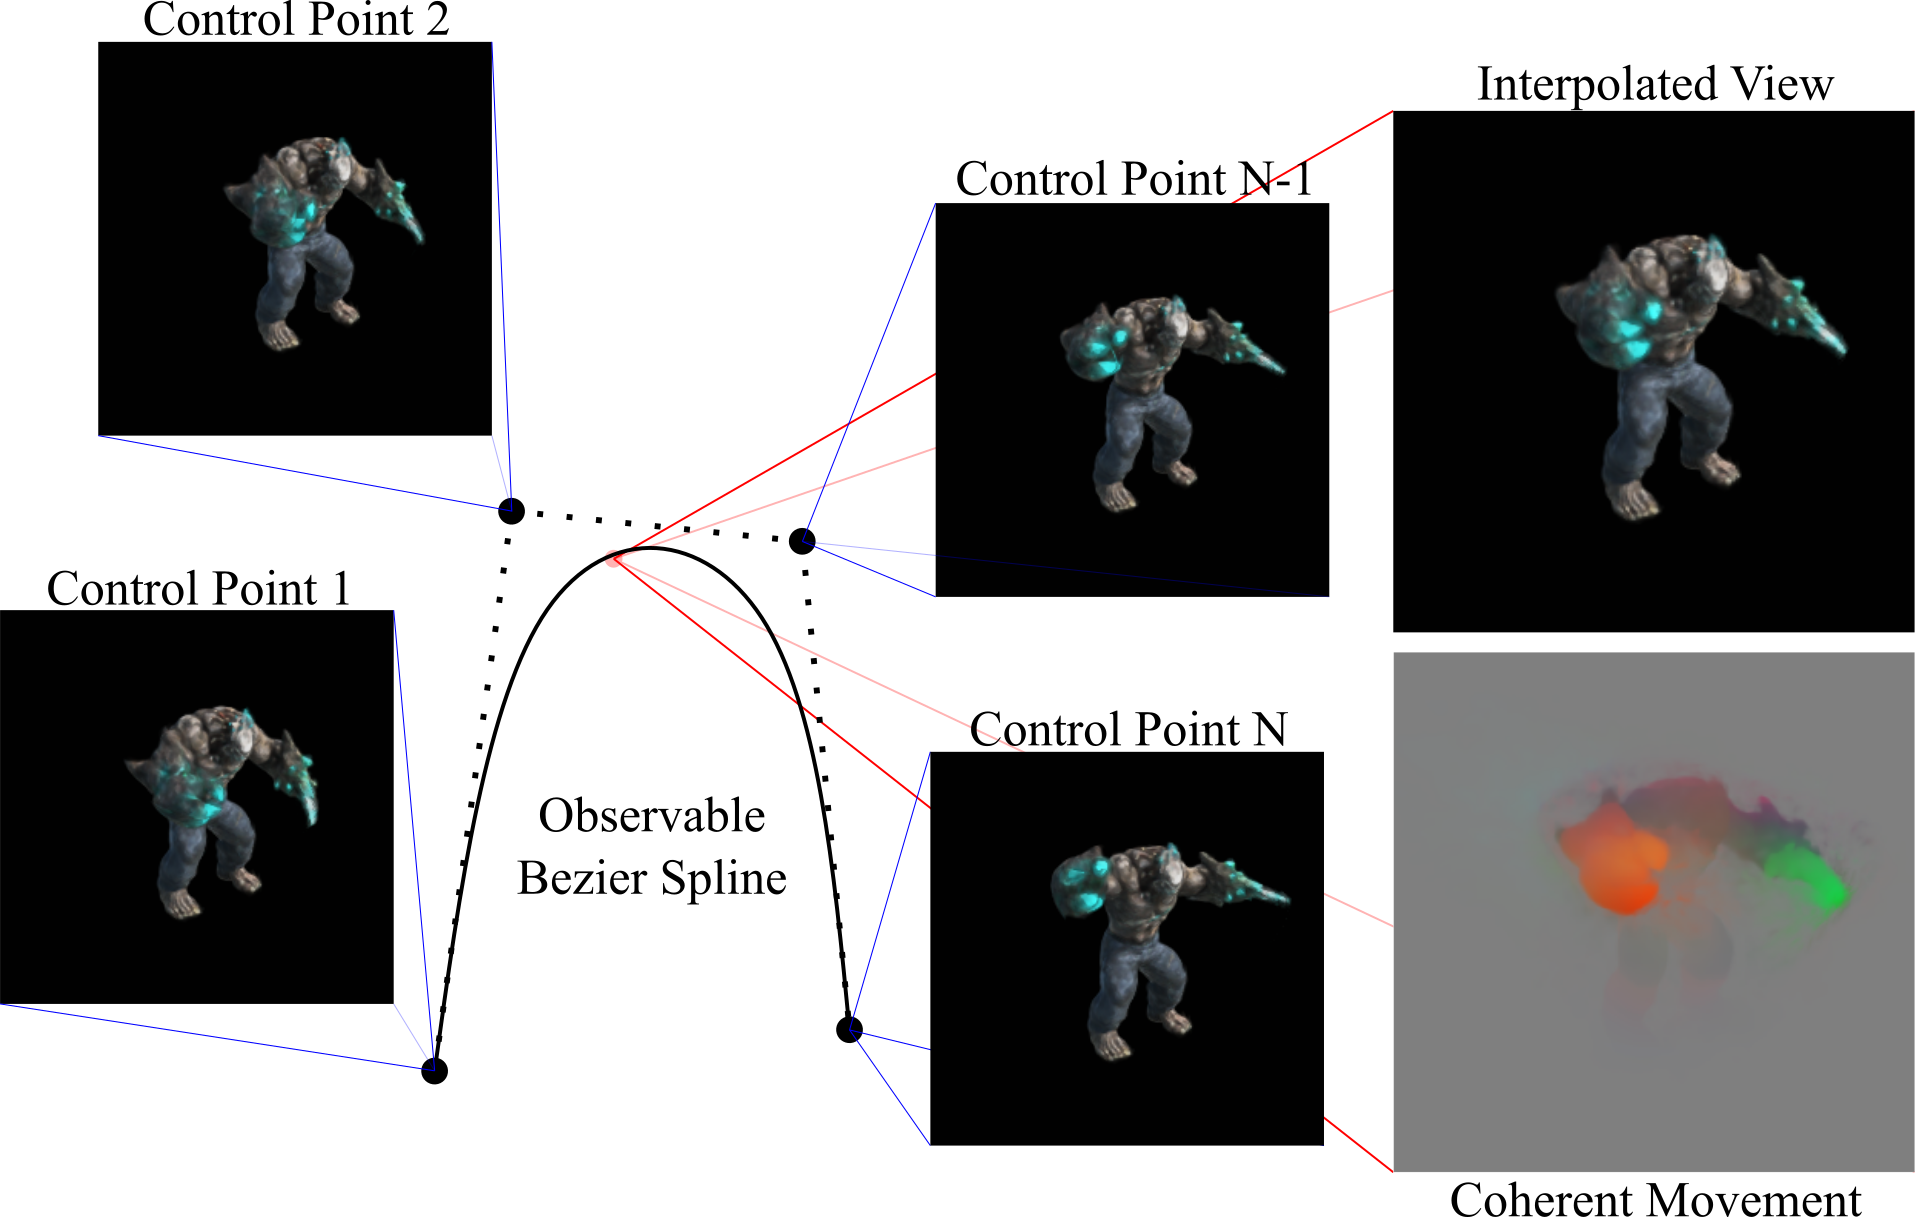
\includegraphics[width=\textwidth]{teaser}
    \caption{
    \label{fig:intro_figure}
    \textbf{Overview of approach.} Conceptually, our approach models movement as interpolation along a high-dimensional bezier spline, where each control point is an object. This is done by learning a function which maps from $x\in\mathbb{R}^3$ to a Bezier spline with $N$ control points. In the figure above, only the first and last control points are visible while rendering. Using this classical formulation, we impose a strong prior on continuity of movement, while enforcing that it is smooth. We compare our model to an implementation of NR-NeRF~\cite{tretschk2021nonrigid}, and find our model is on par qualitatively and produces more coherent movement. A qualitative difference can also be seen in videos comparing the two reconstructions, due to the difference in the velocity of movement.
    }
    \vspace{-3mm}
\end{figure}

\section*{Introduction}

Learning continuous, smooth, functions is a key problem in machine learning, as many problems
are framed as finding good interpolations between a few data points, where we define continuity as $\lim\limits_{x\to c}f(x) = f(c)$.
The continuity of a learned model is not guaranteed, and is enforced through regularization of the output, either by having enough training samples in a short time, or
using regularization such as total variation across time. Since consistency is dependent on data and regularization, it cannot be guaranteed, but only empirically demonstrated. This leads to difficulties in interpolating between sparse training data, and the possibility for sudden changes in output between training points, such as suddenly jumping from one frame to the next in a learned video.
To enforce continuity, we are interested in constructing functions with $C^0$ continuity. $C^0$ continuity is a useful property for many tasks, such as in reconstructing movement to ensure that an object cannot warp between two points instantaneously. We are also interested in $C^1$ continuity, or that the derivative of a function is continuous on some domain. This is because it is not physically possible for an object to instantly change its velocity, therefore reconstructions must have $C^1$ continuity for plausible movement.

To demonstrate how to construct functions with these properties, we tackle the problem of dynamic scene reconstruction using NeRF~\cite{mildenhall2020nerf}, which is a recent method for reconstructing scenes. Following previous work, we define a static scene, which is referred to as the canonical scene, and a model which can produce deformations to the canonical scene. Our approach is a small modification to prior work: to represent the canonical scene, we use a NeRF~\cite{mildenhall2020nerf}, and the deformation model used to model movement is our proposed learned approach. The general approach of deformation networks has been shown to be effective at reconstructing synthetic scenes with movement as in D-NeRF~\cite{pumarola2020dnerf} and real scenes in NR(non-rigid)-NeRF~\cite{tretschk2021nonrigid}. These works show convincing
reconstructions of moving scenes, allowing for novel view synthesis from video. These methods do not have an analytic form, relying purely on learned components but we would like to be able to analyze and modify the movement. For example, an application may want to cluster movement, or change directions, but prior work does not immediately provide a method for doing so. In contrast, classical animation tools are designed to allow for control of movement.

To this end, we look to existing tools in animation for creating realistic movement while allowing a high-degree of control for artists and animators. For example, there are tools such as keyframing and splines, which allow animators to construct movement with a small set of tunable knobs. Despite few degrees of freedom, these tools allow artists and animators to breathe life into animation, with a high degree of control. In addition, mathematical constructs such as splines have also been thoroughly studied to understand their behaviour and how they can be manipulated, and thus are modifiable in post-processing.

Thus, we use the animation techniques of Bezier splines as a method to enforce continuous interpolation in Dynamic NeRF, finding that we are able to get comparable performance without additional cost in memory, and the desired properties of $C^0, C^1$ continuity.
In summary, our contributions are as follows:

\begin{enumerate}
    \item A general architecture for $C^0, C^1$ continuity over a continuous domain.
    \item An application of this architecture building on NR-NeRF to enforce continuity of movement with an analytic form with negligible computational cost, while performing on par with the original.
\end{enumerate}

\begin{figure}
    \vspace{-6mm}
    \centering
    \begin{minipage}[c]{0.5\textwidth}
    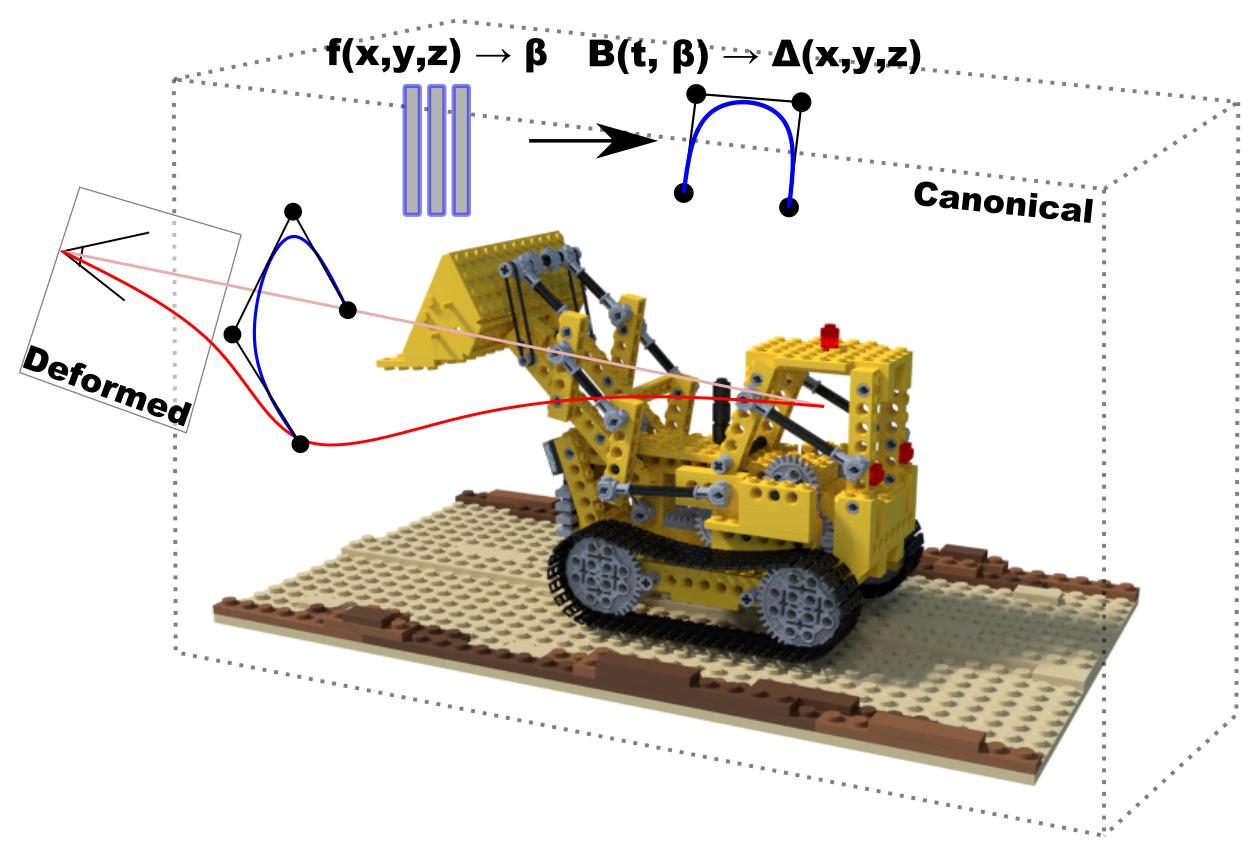
\includegraphics[width=\textwidth]{spline_nerf_diagram.png}
    \end{minipage}
    \begin{minipage}[c]{0.45\textwidth}
    \caption{
        \label{fig:arch_diagram}
        \textbf{Spline-based Dynamic NeRF}. Instead of using an MLP to directly predict ray-bending, $x' = \Delta(\text{MLP}(x, t)) + x$,  at a given time, we predict a set of Bezier spline control points. Then, we use the Bezier spline defined by these points to interpolate position based on time: \newline $x' = \Delta(B(\beta,t)) + x$, where $B$ is a Bezier spline parametrized by $\beta = \text{MLP(x)}$.
    }
    \end{minipage}
    \vspace{-10mm}
\end{figure}

\iffalse
\begin{figure*}
    \centering
    \begin{minipage}[b]{0.45\textwidth}
    \centering
    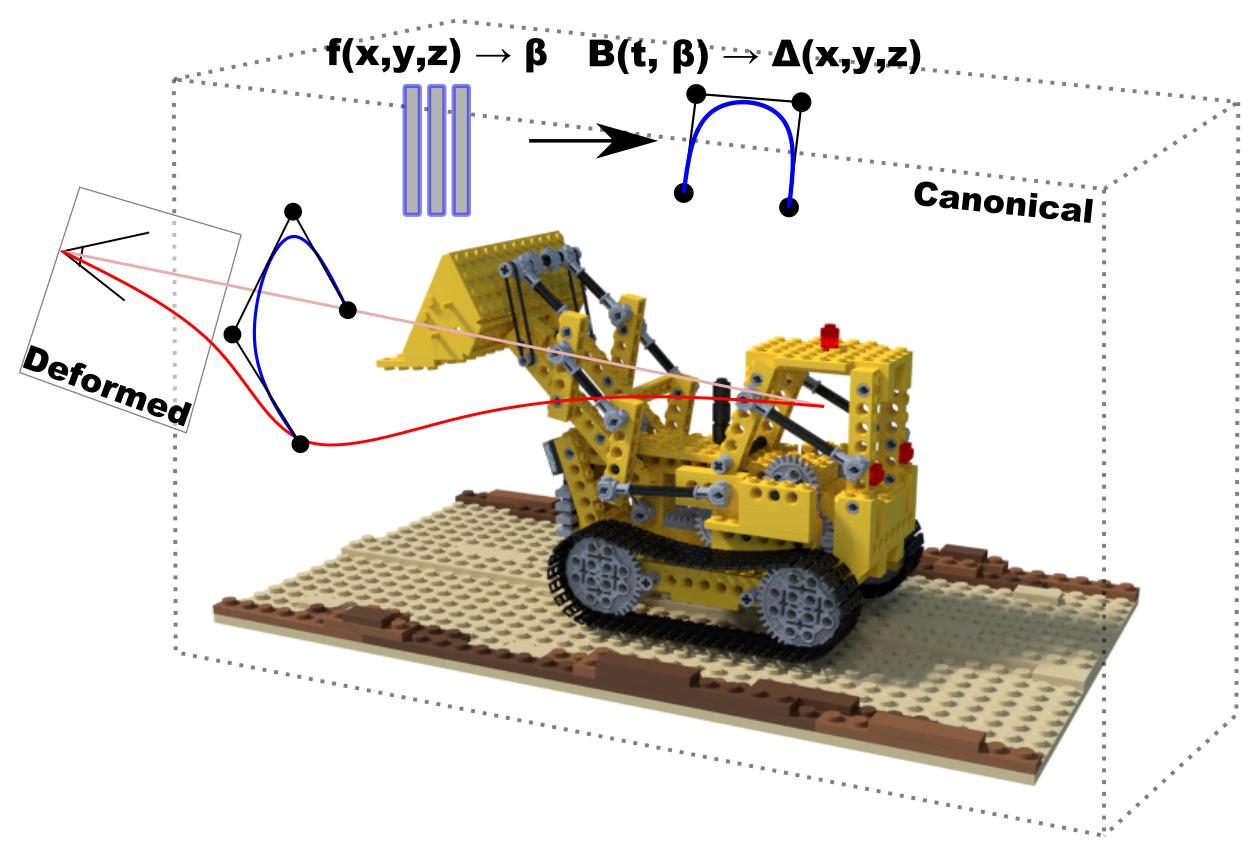
\includegraphics[width=\textwidth]{spline_nerf_diagram.png}
    \caption{
        \textbf{Spline-based Dynamic NeRF}. Instead of using an MLP to directly predict ray-bending, $x' = \Delta(\text{MLP}(x, t)) + x$,  at a given time, we predict a set of Bezier spline control points. Then, we use the Bezier function defined by these points to interpolate position based on time: $x' = \Delta(B(\beta = \text{MLP}(x),t)) + x$.
    }
    \label{fig:arch_diagram}
    \end{minipage}\hfill
    \begin{minipage}[b]{0.45\textwidth}
    \centering
    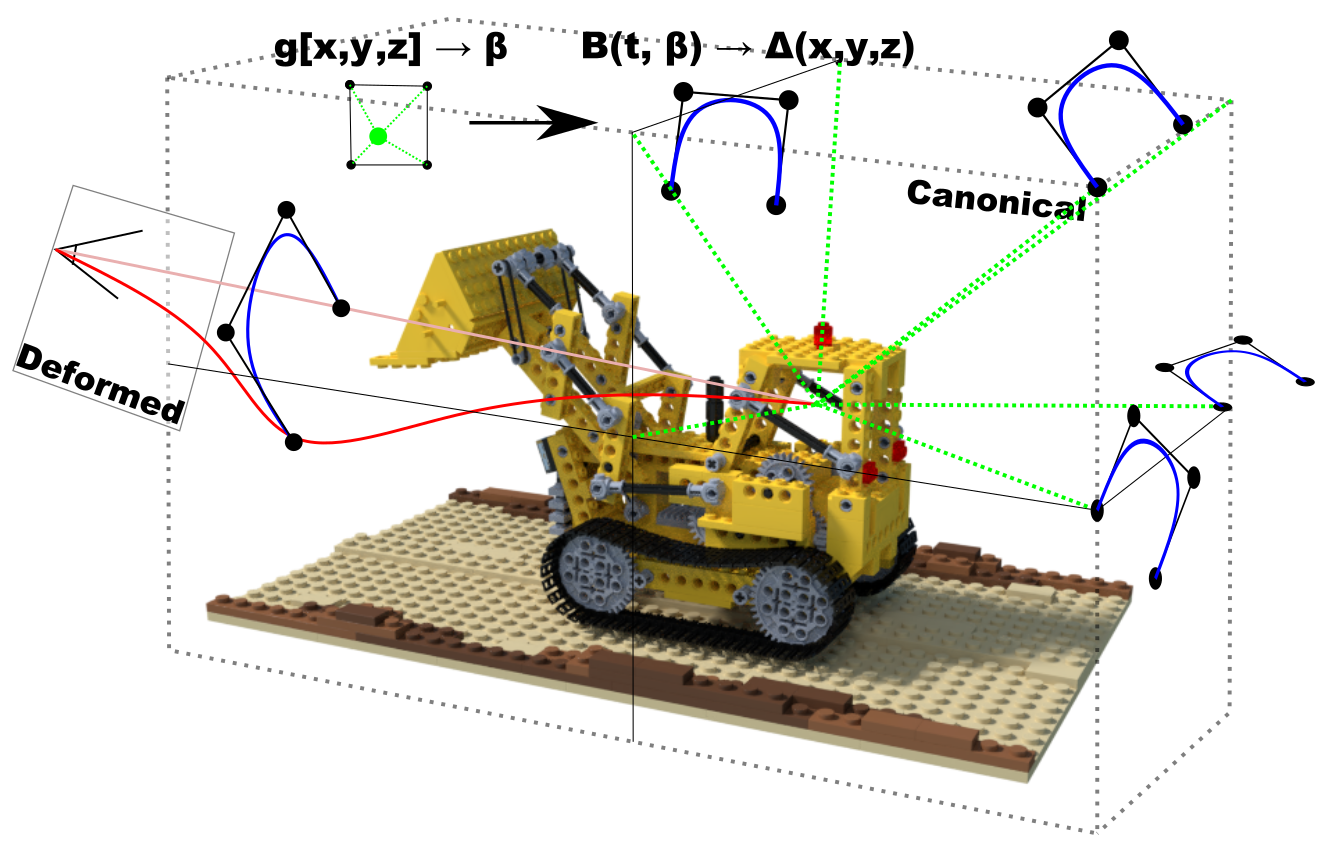
\includegraphics[width=\textwidth]{c0_paper/voxel_spline.png}
    \caption{
        \label{fig:voxel_diagram}
        \textbf{Voxelized spline-based Dynamic-NeRF}. We also propose a voxelized model for Dynamic-NeRF, to demonstrate that our method could be extended to reconstruct sparse scenes rapidly. At each voxel coordinate, we store an additional set of control points which are used for ray-bending. This allows us to efficiently and sparsely bend rays, without needing to query an MLP. Our implementation shares much of the same code as the MLP-based approach, but has better memory usage.
    }
    \end{minipage}
\end{figure*}
\fi
\section*{Related Work \& Background}

\subsection*{Static Scene Reconstruction}

Static scene reconstruction is the problem of reconstructing a 3D model from a set of 2D views.
Neural Radiance Fields (NeRFs)~\cite{mildenhall2020nerf} are a recent technique for reconstructing new views of a scene from new camera positions. To represent highly-detailed scenes, NeRFs model a scene as a continuous volume of varying density, which emits different colored light depending on the view direction. This is based on traditional volume rendering techniques:
\[ I(r) = \int_{t_n}^{t_f} T(t, r) \sigma(r(t)) c(r(t), r_d)dt, \]
where 
\[ T(t, r) = \exp(-\int_{t_n}^{t} \sigma(r(s))ds), \]
\noindent
where $I(r)$ is the illumination along camera ray $r(t) = r_o + r_d t$, $r_o, r_d$ are the ray origin and direction respectively, and $t$ is some positive distance along the ray. NeRFs are able to accurately reconstruct high-frequency features by recovering $\sigma$, the density at a given point, and $c$, the view-dependent color at a given point by modelling them as MLPs with an additional encoding scheme that can differentiate between extremely close points. NeRFs evaluate the above equations by performing ray-marching and computing $T(j,r) = \Sigma -\exp\sigma_i c_i$, by partitioning the ray into evenly spaced bins and sampling randomly from within each bin. There has been a plethora of work exploring NeRF and extensions which permit capturing more variance.

There have been a significant number of extensions to NeRF, including optimizations on the encoding for differentiating positions in space~\cite{tancik2020fourfeat}, better sampling approaches~\cite{barron2021mipnerf}, faster training~\cite{yu2021plenoxels}, and more~\cite{sitzmann2019siren}.

\subsection*{Dynamic NeRF Reconstruction}

Dynamic scene reconstruction is removing the assumption in static scene reconstruction that all views are under the same condition, such as the same lighting and that nothing has moved.
NeRFs were designed to only handle static scenes, and thus cannot accurately reconstruct scenes which contain movement, alternative lighting conditions, or other changes between frames.
In order to model dynamic scenes, there have been two diverging approaches.

One kind of approach directly models the transformation in the time domain, by learning a function $\sigma(x,t)=f(x\in\mathbb{R}^3, t\in[0,1])$, which include works such as HyperNeRF~\cite{park2021hypernerf}, NeRFies~\cite{park2021nerfies}, Space-Time Invariant Irradiance Fields~\cite{xian2021space}, and others~\cite{Wang_2021_CVPR,du2021nerflow}. By directly modelling the variation of the density, these methods are able to reconstruct large deformations in latent spaces and reconstruct a wide variety of transformations from a single radiance field. These often allow for fun transformations in some learned space between many similar scenes, which allow novelty warping and interpolation.

The other kind of approach models movement directly as translation. NeRFs are not able to move the objects inside the scene since we can only evaluate the NeRF at a given $x$. Instead we bend the rays, warping what is visible from a given view. This is essentially a perspective shift of a transformation of the space being rendered. Instead of moving an object that is seen by ray $r$, we warp ray $r$ such that it is sees the object. The equation for density is defined as $\sigma(x,t)=f(x+\Delta(x,t))$. This formulation enforces a coherent canonical representation, while directly modelling movement, and has been shown to be able to reconstruct both synthetic scenes with D-NeRF~\cite{pumarola2020dnerf} and real scenes in NR-NeRF~\cite{tretschk2021nonrigid}. There has also been work on recovering movements of entire NeRFs within a scene, such as in \cite{dynamicSceneGraphs}, but this work diverges from that approach as we are interested in reconstructing movement within a NeRF.

We note that a lot of prior work in this field not been peer-reviewed~\cite{pumarola2020dnerf,li2021neural,park2021nerfies,neural3dViewSynthesis}, but these works still have a significant impact, especially since the field moves quickly.

The pros of directly including time as a function in the MLP are that we are able to represent a much broader class of functions, in theory every frame may be fully distinct from the previous, but the movement formulation lends itself to smoothness between frames. Our approach falls into the movement category, as we are interested in accurately reconstructing smooth movement as opposed to generalizing over many classes of transformations.

\subsection*{Bezier Curves}

Bezier curves refer to a specific set of polynomials parametrized by a set of control points. They are most commonly used as cubic polynomials: $f(x) = ax^3 + bx^2 + cx + d$,
where $x$ is the variable we are interested in interpolating over. An example of a Bezier Spline is shown in Figure~\ref{fig:bezier_diagram}. The general formulation for
the Bezier basis functions is defined as $B^n(t) = \Sigma^n_{i=0}
{n \choose i} (1-t)^{n-i} t^i$ where $n$
is the degree of the Bezier polynomial. In order to give control of the Bezier curve, we
introduce "control points", which weigh different points along the curve differently:
$B^n(t) = \Sigma^n_{i=0} P_i {n \choose i} (1-t)^{n-i} t^i$, where $P_i\in\mathbb{R}^3$ for 3D
movement. For a more comprehensive guide on Bezier splines, we refer the reader to a more
\href{https://pomax.github.io/bezierinfo/index.html}{complete reference}~\cite{bezier_primer}.

\begin{figure}
    \centering
    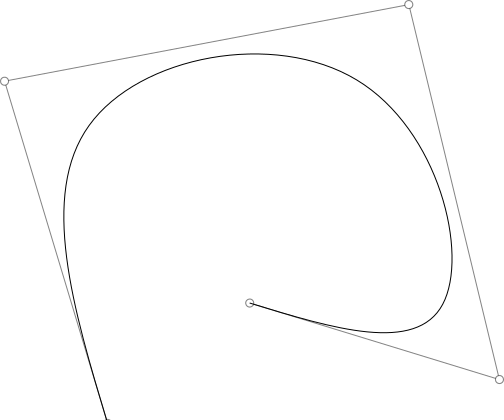
\includegraphics[width=0.2\textwidth]{bezier_curve.png}
    \caption{
        \textbf{Example of a Bezier Spline}.
        Bezier curves are a low-dimensional polynomial representation that allows for smooth interpolation between a few control points. We reconstruct control points to produce smooth movement and induce a prior on continuity. Bezier curves are common in both animation and drawing software.
    }
    \label{fig:bezier_diagram}
\end{figure}


\section*{Method}

Our design imposes additional structure on top of existing machine learning
approaches, enforcing properties on the reconstructed values. For functions \[ f(p, t)\to\mathbb{R}^n, t\in[0,1] \] which is modelled through
a learned approach, we decompose it into a function: \[ f(p)\to\mathbb{R}^{n\times O}, B_O(f(p), t)\to\mathbb{R}^n
\] Where
$O$ is the order of the Bezier spline, $f(p)$ is the learned control points, and $B_O(f(p), \cdot)$ is the evaluation
of the $O$th order Bezier spline with control points defined by $f(p)$.

\subsection*{Architecture}

Specifically for dynamic NeRF, $f(p)$ is defined as
$\text{MLP}(x,y,z)\to\mathbb{R}^{3\times O}$. We ray march from a camera with known position and
view direction through the scene, and at every point we compute the set of control points for a Bezier curve. We then evaluate the Bezier curve at a given time, and deform the ray by the result, producing some $\Delta_0(x)$. The number of spline points for the Bezier curve is hyperparameter, but we are able
to accurately reconstruct movement with as low as 4 spline points, but experiment with 16 spline points. In order to evaluate the Bezier curve in a numerically stable way, we use De Casteljau's
algorithm. In a future extension, we plan on extending it to handle rational Bezier splines, which would allow for even greater control of movement.

De Casteljau's algorithm evaluated at time $t$ is characterized by the recurrence relation:
\[ \beta_i^{(0)} = \beta_i, \]
\[ \beta_i^{j} = (1-t)\beta_i^{(j-1)} + t\beta_{i-1}^{(j-1)}, \]
which can be thought of as linearly interpolating between adjacent control points until there is only a single point remaining. This takes $O(n^2)$ operations to evaluate, where $n$ is the number of control points.

We are also interested in constructing a reasonable canonical NeRF, and arbitrarily select $t = 0$ to be canonical. Thus, we are interested in Bezier Curves where $B_O(0) = \overrightarrow{0}$. This can be achieved in two different ways, either by assigning $p_0 = \overrightarrow{0}$, and only computing the other control points: $f(p) = p_{1\cdots O-1}$. Then, we can use the Bezier spline with the control points as the concatenation of $\overrightarrow{0}$ with the other control points: $[\overrightarrow{0}, p_{1\cdots O-1}]$. Alternatively, we can compute $p_{0\cdots O-1}$ and use the Bezier spline with control points but subtract the first predicted point from all of them: $[p_{0\cdots O-1}]-p_0$, and the final change in position is $\Delta_0(x) = B_O(f(p)-f(p)_0,t)+p_0$. While both formulations are in theory equivalent and explicitly concatenating $\overrightarrow{0}$ leads to fewer degrees of freedom, we find the second approach leads to better convergence near $t=0$, so we use that.

Following NR-NeRF, we also learn how rigid each ray is, which in theory should allow more efficient learning of which regions are space are fixed. This rigidity $\in[\epsilon, 1]$)is computed as a function of position:
\[ \text{Rigidity} =\sigma_{\epsilon^\uparrow}(\text{MLP}(x)), \]
\[ \sigma_{\epsilon^\uparrow}(v) = \sigma(v)(1-\epsilon) + \epsilon, \]
where $\sigma$ is defined as the sigmoid function $\frac{1}{1+e^{-x}}$. Rigidity rescales the
difficulty of learning movement, making it more easy to represent and classify static scene
objects. The final change in position is defined as $\Delta(x) = \text{Rigidity}\times
\Delta_0(x)$.

In order to reconstruct RGB values, we also diverge from the original NeRF, and only allow for
positional dependent colors:
\[ \text{RGB} = \sigma_{\epsilon-\text{wide}}(\text{MLP}(x)) \]
\[ \sigma_{\epsilon-\text{wide}}(v) = \sigma(v)(1+2\epsilon) - \epsilon \]
using the activation function as described in MIP-NeRF~\cite{barron2021mipnerf} in order to prevent vanishing gradients on colors. Because of the low number of
samples for a moving object at a given view, it is more difficult to learn specular
reflection, thus it leads to better convergence to model the diffuse color of an object. This is in line with NR-NeRF and D-NeRF, which also model the diffuse component.

\iffalse
\subsection*{Loss}

While training, we introduce another loss term, as the $\ell_2$ loss may have
difficulty when there is a large pixel-wise gap in movement between the learned and predicted
component. $\ell_2$ may also miss large structural differences between two images if they are close in color, so we add a loss function which is high for incorrect structure of an image.

The new loss term is \[
    L_\text{FFT} = \text{MSE}(\text{FFT}(I_\text{GT}), \text{FFT}(I_\text{predicted}))
\],
where the FFT is the 2D fast Fourier transform of an image.
MSE is the mean squared error in the complex domain as the FFT has both a real and imaginary component, and is defined as \[ \text{MSE}(a\in\mathbb{C}^k,b\in\mathbb{C}^k) \]
\[ = \frac{1}{k}\Sigma_{i=0}^k|a_i-b_i| \]
\[ |z\in\mathbb{C}| = (\Re(z)+\Im(z))(\Re(z)-\Im(z)) \]
We introduce this term as a cheap replacement to structural similarity (SSIM), since the
FFT captures information about the structure of the whole image, which is useful in a dynamic setting due to the disjointedness of where a predicted object may be as opposed to its final position\footnote{In a published iteration, we would likely perform an ablation of this loss function.}.

Our final loss formulation is:
\[ \ell_2(I_\text{predicted}, I_\text{GT}) + L_\text{FFT}(I_\text{predicted}, I_\text{GT}) \]
without any additional regularization terms.

Our formulation is simpler compared to NR-NeRF since there is no need to regularize
temporal consistency, making the optimization process simpler. Our training process also does not require adding in additional frames over time for short sequences, so we randomly sample from all available frames. This is contrast to D-NeRF, which requires adding frames in during training since it has to enforce that at $t=0$ the predicted movement is 0.

\subsection*{Training}

For training, we sample random crops of random frames, computing the loss defined previously and back-propagating through the whole network. We use autograd to optimize control points and the canonical NeRF jointly, but note that there are also classical approaches to solving spline points which may lead to faster optimization in the future. We use the Adam optimizer~\cite{Kingma2015AdamAM} with cosine simulated annealing~\cite{loshchilov2017sgdr} to go from $\num{2e-4}$ to $\num{5e-5}$ over the course of a day.

For some scenes, we are able to have higher learning rates, but for much darker scenes it's necessary to lower the learning rate to converge.

\subsection*{Long Duration $C^0$ Continuity}

While the above structure is sufficient to model short-term $C^0$ continuity, it runs into
numerical instability and higher cost the longer the sequence is, due to the $O(n^2)$
evaluation cost of De Casteljau's algorithm. To deal with this, we design an additional architecture which
composes the previous architecture for many small $C^0$ curves. Concatenating many small splines permits for reconstruction of infinitely long sequences with guaranteed $C^0$-continuity with only a few additional models.

The architecture is based off of poly-splines, or a composition of many small Bezier splines.
For a known-length sequence, we divide it into $K$ segments, and assume that $K$ evenly divides the total number of frames. We can then treat $t$ as is
in the range $[0, K]$, and $t$ can be decomposed into a segment number and fractional component:
\[ k\in\mathbb{Z}_K=\lfloor t\rfloor, t'\in[0,1)=t-k \]
Then we define an embedding $\text{Emb} = \mathbb{R}^{Z\times(K+1)}$, where $Z$ is a latent
dimension size. We then create an "anchor" network:
\[
    \textit{anchor}(x\in\mathbb{R}^3,z\in\mathbb{R}^Z) = \text{MLP}(x,z)\to(\mathbb{R}^3,\mathbb{R}^{Z'})
\]
We call it an "anchor" network because it computes
endpoints which anchors each of the curves, and also computes a representative latent vector. Between these two
endpoints, we are interested in computing $O-2$ intermediate spline points. We define the
control point estimation network as
\[
\textit{control}(x\in\mathbb{R}^3, z_1, z_2\in\mathbb{R}^{Z'}) = \text{MLP}(x,z_1,z_2)\to\mathbb{R}^{O\times\mathbb{R}^3}
\]
Where $z_1,z_2$ are the
representative latent vectors from the anchor network, and it outputs $O-2$ spline points in
$R^3$. We can also include a per-segment rigidity value, similar to above, but lose
some guarantees of continuity by doing so.

In order to evaluate the network at a given time $t$ and other inputs $x$, we first compute $k, t'$. Then, we compute
the anchor points at
\[ p_0,z_1=\textit{anchor}(x,\text{Emb}[k]) \]
\[ p_\text{end},z_2=\textit{anchor}(x,\text{Emb}[k+1]) \]
and the intermediate control points as \[ p_{1\cdots O-2} = \text{control}(x,z_1,z_2) \]
The final set of control points we use
is the concatenation of the anchors with the intermediate points:
$[p_0, p_{1\cdots O-2}, p_\text{end}]$. Using this set of control points, we evaluate the Bezier
curve spline at $t'$ using De Casteljau's algorithm:
\[ \text{De Casteljau}([p_0, p_{1\cdots O-2}, p_\text{end}], t) = \Delta(x) \]
Because we are evaluating adjacent embeddings ($k, k+1$) for each anchor, we are guaranteed that the endpoints between each spline segment are identical. Information is also carried over between segments through the anchor's
representative latent vector, allowing the network to maintain velocity between curves if necessary.

This architecture enforces a guarantee of consistency, regardless of how long a reconstructed signal is. It also naturally allows movement at one time to be distinct from another,
as while the endpoints of the spline are fixed, movement defined by the intermediate control points is allowed to be fully independent of other
segments. While we construct this architecture for long dynamic sequence reconstruction, we argue that it works more generally for generating $C^0$-continuous functions in any domain.

One obvious question is why a more complex architecture is necessary as compared to predicting all spline points and using only some of them. In the case of extremely long sequences, the number of spline points may increase linearly with the length of the function, and for dynamic NeRF we would have memory cost of $O(H\times W\times D\times t)$ which is prohibitively expensive. With the proposed architecture, we are able to sample sparsely, maintaining a constant memory usage with respect to time.

We do yet not demonstrate the effectiveness of the architecture, due to time constraints, and the author's incompetence\footnote{If this were to be published, I would demonstrate this architecture, but cannot due to time constraints.}.
\fi
\section*{Results}

In order to demonstrate that our method works, we run it on D-NeRF's synthetic
dataset which contains 8 different rendered scenes. These scenes have ground truth camera positions and viewing directions, as well as timestamps. They capture physically plausible movement, so there are no discontinuities or jumps between frames.

While we do not demonstrate our method on any real datasets, our approach does not have any limitations that would prevent it from doing so as compared to D-NeRF. Given that a real dataset would have to strictly abide by physics, the bias introduced by enforcing continuity should force our model closer to correctness than D-NeRF.

\subsection*{Quantitative Results}

The Spline-NeRF is able to perform on par with D-NeRF on their synthetic dataset, and slightly outperforms it in some cases. This is likely because D-NeRF can predict non-realistic movement, such as jumping from frame-to-frame, or suddenly accelerating. In practice, D-NeRF learns fairly smooth movement, but quantitatively looks different from our methods movement, which is likely due to variations in velocity and acceleration of the learned approach. By using Bezier splines, we enforce that movement is fluid and can better reproduce missing frames. This leads to a small improvement in PSNR, because the dataset contains simple movement, but we expect that in longer sequences or data with large gaps this difference would be more visible.

\subsection*{Qualitative Results}

The difference between our work and D-NeRF can be observed in the difference of flow between scenes. It can be observed from Fig.~\ref{fig:dnerf_cmp} that our method more accurately captures squashing and stretching of movement, as the top of the ball is not moving but the bottom of the ball is falling. In contrast, D-NeRF contains approximately equal flow for the entire ball.

The difference between the two is also more clearly seen in videos of reconstruction. Spline-NeRF visibly has the effect of tweening between views, slowing into stops, while D-NeRF has more less smooth starts and stops.

\begin{table*}[t]
    \centering
    \begin{tabular}{|c| c|c | c|c | c|c | c|c |}
    \hline
    \textbf{PSNR$^\uparrow$ $|$ MS-SSIM$^\uparrow$} & \multicolumn{2}{c|}{Bouncing Balls} & \multicolumn{2}{c|}{Hellwarrior} & \multicolumn{2}{c|}{Hook} & \multicolumn{2}{c|}{Jumping Jacks} \\
    \hline
    D-NeRF & \textbf{26.139} & \textbf{0.974}
           & 33.314 & 0.968
           & 27.954 & 0.978
           & 27.610 & 0.979 \\
    \hline
    Spline-NeRF & 25.139 & 0.967
               & \textbf{33.504} & 0.968
               & \textbf{28.104} & \textbf{0.979}
               & \textbf{27.756} & \textbf{0.981} \\
    \hline
    & \multicolumn{2}{c|}{Lego} & \multicolumn{2}{c|}{Mutant} & \multicolumn{2}{c|}{Standup} & \multicolumn{2}{c|}{T-Rex} \\
    \hline
    D-NeRF & \textbf{23.409} & \textbf{0.934}
           & 28.833 & 0.979
           & 31.307 & 0.989
           & \textbf{25.734} & \textbf{0.978} \\
    \hline
    Spline-NeRF & 23.302 & 0.933
               & \textbf{29.222} & 0.979
               & \textbf{31.349} & \textbf{0.990}
               & 25.421 & 0.973 \\
    \hline
    \end{tabular}
    \vspace{3pt}
    \caption{
        \textbf{Metric comparison of Spline-NeRF to D-NeRF.}
        Bezier splines are able to recover movement with slightly improved accuracy in dynamic scenes as compared to D-NeRF~\cite{pumarola2020dnerf}. Despite, or maybe because of, the forced prior of continuous movement, we are able to learn a smooth interpolation through each frame. We randomly samples all frames from the start of training, as opposed to D-NeRF which requires slowly introducing new frames, but we also remove the constraint that at time 0 D-NeRF must have no movement. Here, we parametrize Spline-NeRF with 6 control points.
    }
\end{table*}

\begin{figure*}
    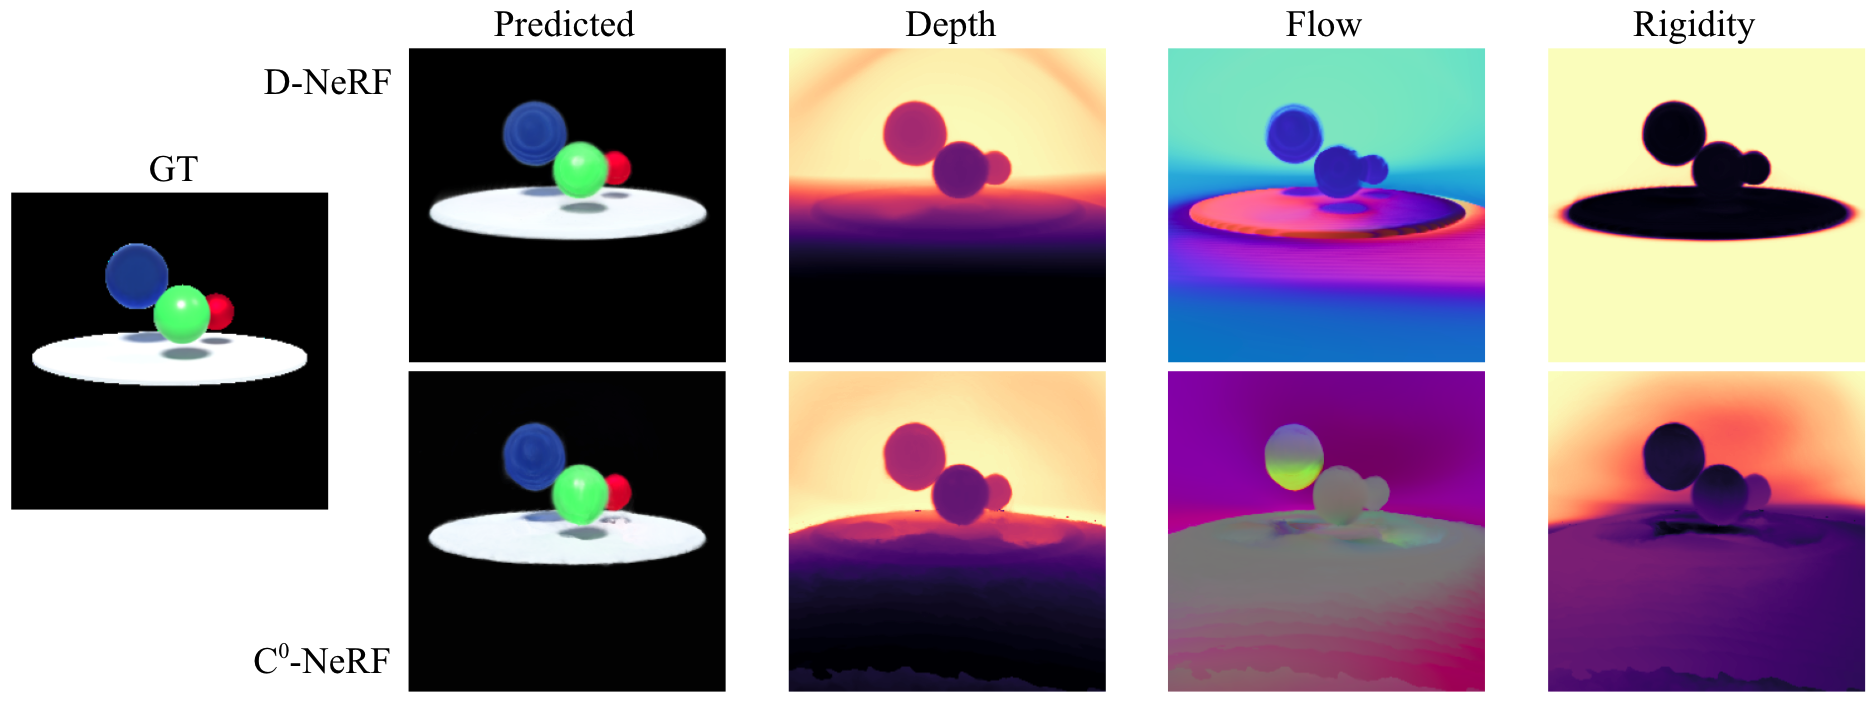
\includegraphics[width=\textwidth]{dnerf_compare}
    \caption{
        \label{fig:dnerf_cmp}
        \textbf{Visual comparison of Spline-NeRF to D-NeRF.}
        Results comparing movement in D-NeRF~\cite{pumarola2020dnerf} versus Bezier-splines for a small timestep. There is substantial difference in the predicted flow, since D-NeRF cannot guarantee the initial frame has no movement. There is also a significant difference in rigidity, which is not easily explained. We believe it may be significantly easier to model low movement with splines, thus there is less of a need for rigidity.
    }
\end{figure*}

\section{Discussion}

Our method produces coherent movement in objects without explicit regularization, and is able to
converge much faster as compared to prior work. It also does not suffer extremely significant
around time extremities as compared to D-NeRF, since we are analytically able to ensure that at
time 0 there is no motion.

In addition, our method demonstrates extremely smooth interpolation, as enforced by the network.
We are thus able to exaggerate movements significantly. Also because of the analytic nature
of splines, we are likely able to perform interesting motion deformations, such as diverging
motion paths in order to construct novel motion.

One issue with our approach is that because it is forced to learn continuous representations, it
has some difficulty when surfaces collide and bounce apart, as it must separate each surface but
the boundary between them may be very small and thus hard to distinguish.

\section*{Conclusion}

In conclusion, we devise a new architecture for $C^0$ continuous interpolation, and demonstrate
that it works on Dynamic Neural Rendering. Our architecture is able to accurately and quickly
reconstruct scenes, while providing stronger guarantees with a well understood tool.
Hopefully, this inspires more introduction of classical tools inside of the differentiable rendering pipeline.

While our work is incremental, requiring very little code, because it changes the underlying structure there are a significant number of extensions that can be done with it.

\section*{Future Work}

For future work, we plan on applying Bezier splines to other signals, such as sound for
reconstruction of long music. Sound must be continuous, even if it has sharp changes, and may change significantly over time, so our architecture is suitable for its reconstruction.

Another next step in neural rendering is to encode this using a Plenoxel~\cite{yu2021plenoxels} or another sparse structure, to allow for rapid training of dynamic scenes. To the author's knowledge, there is no real-time construction of 3D scenes since there did not exist a deep-learning approach to reconstructing movement. Bezier splines fill in this gap, and since they only require a fixed number of parameters, this should allow for efficient rendering and training without requiring an MLP evaluation. If this follows the trend of scene reconstruction, it may be on the order of 100 times faster to reconstruct dynamic scenes, without any loss in quality, and we hope that our work gets adopted for this purpose.

It may also be interesting to explore different formulations of splines, as we only select
Bezier splines due to ease of implementation, but it may be that other splines might be more
numerically stable or have stronger expressivity for reconstruction.

\section*{Acknowledgements}

Thanks to Elliot Cuzzillo for helping proofread this work.

{\small
    \bibliographystyle{splncs04}
    \bibliography{ref}
}

\end{document}